\newpage
% ============================================================
\section{Actividad 6: Fractalidad en tráfico transaccional Cloud}
% ============================================================

% ------------------------------------------------------------
\subsection{Contexto: un arco transversal}
% ------------------------------------------------------------

El arco analítico desarrollado en las actividades previas sigue una progresión
metodológica deliberada. Las Actividades~1 y~2 validaron las propiedades
estadísticas de los estimadores Varianza--Tiempo y Log--Escala sobre secuencias
sintéticas de referencia: secuencias i.i.d.\ con $H=0{,}5$ como límite de
independencia, y procesos LRD monofractales (\texttt{wfbm}) y multifractales
(\texttt{betamwm}) como banco de prueba controlado. Las Actividades~3,~4 y~5
trasladaron estas herramientas al dominio fisiológico, caracterizando la
estructura fractal de la variabilidad cardíaca y construyendo un clasificador
mono/multifractal con asociaciones clínicas significativas.

La pregunta que orienta esta actividad es de naturaleza transversal: ¿la
fractalidad es un fenómeno exclusivo de sistemas biológicos, o emerge también en
infraestructuras tecnológicas? A diferencia de la fisiología cardíaca, donde la
regulación autónoma produce memoria persistente con $H\approx0{,}96$ y
heterogeneidad multiescala, el tráfico transaccional Cloud opera bajo dinámicas
de usuarios concurrentes, cachés en cascada y ráfagas de solicitudes
correlacionadas. Este hallazgo trasciende el dominio tecnológico: si la
fractalidad aparece tanto en un corazón sano como en un servidor web bajo carga,
debe existir un conjunto de propiedades estructurales comunes que la generen.

% ------------------------------------------------------------
\subsection{Dataset y metodología}
% ------------------------------------------------------------

Se analiza el dataset NASA HTTP, un registro de solicitudes HTTP al servidor web
de la NASA durante los meses de julio y agosto de 1995. La serie objeto de
estudio son los tiempos entre llegadas consecutivas (\textit{inter-arrival
times}), que capturan la dinámica de acceso de miles de usuarios concurrentes.

La serie contiene $975\,721$ muestras con media $\mu = 2{,}7450\,\text{s}$,
mediana $1{,}0000\,\text{s}$ y desviación estándar
$\sigma = 137{,}6685\,\text{s}$. La enorme dispersión (coeficiente de
variación $>50$) es indicio de heterogeneidad estructural: la mayoría de los
intervalos son breves, pero episodios de congestión producen colas de espera de
varios minutos.

\begin{figure}[H]
    \centering
    \begin{minipage}[t]{0.48\textwidth}
        \centering
        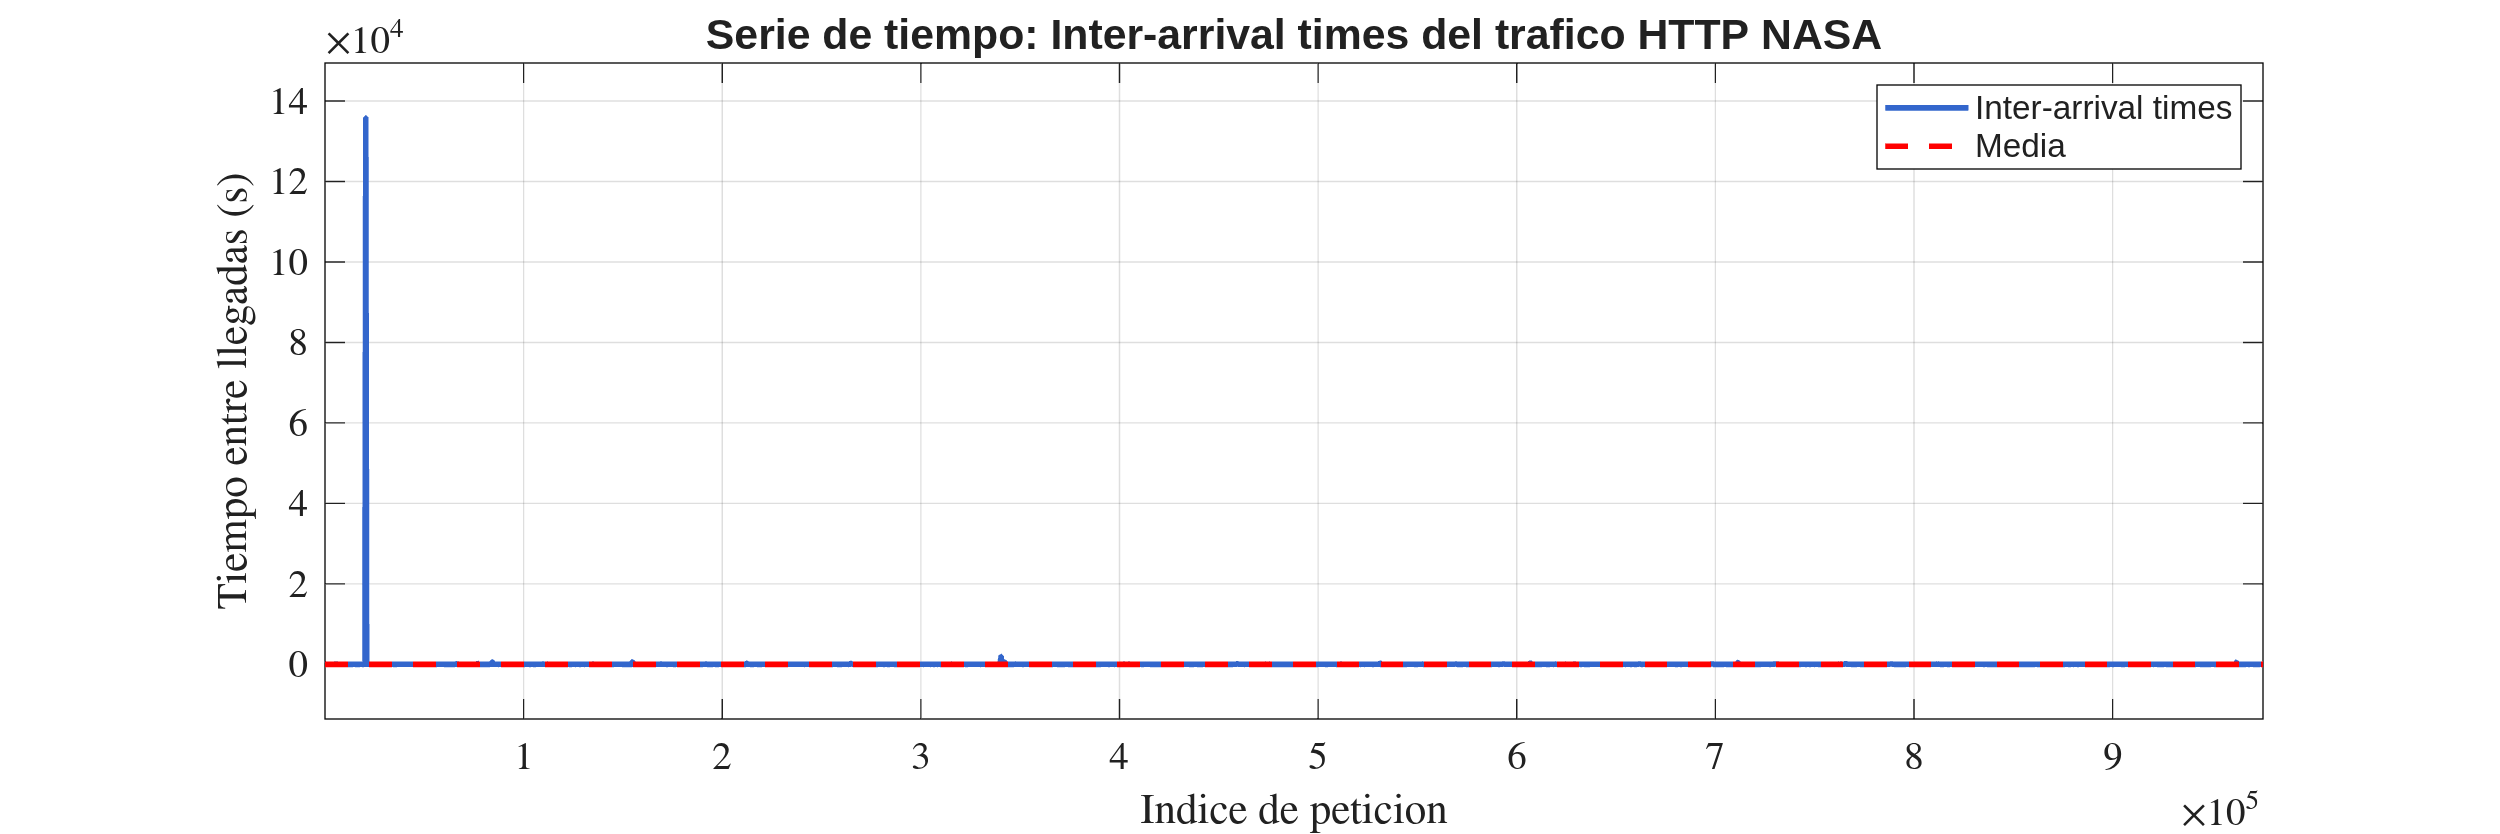
\includegraphics[width=\textwidth]{actividades/actividad6/imgs/serie_tiempo.png}
        \caption{Serie de tiempos entre llegadas del dataset NASA HTTP.
                 Se observan ráfagas intensas seguidas de periodos de
                 actividad reducida.}
        \label{fig:a6-serie}
    \end{minipage}
    \hfill
    \begin{minipage}[t]{0.48\textwidth}
        \centering
        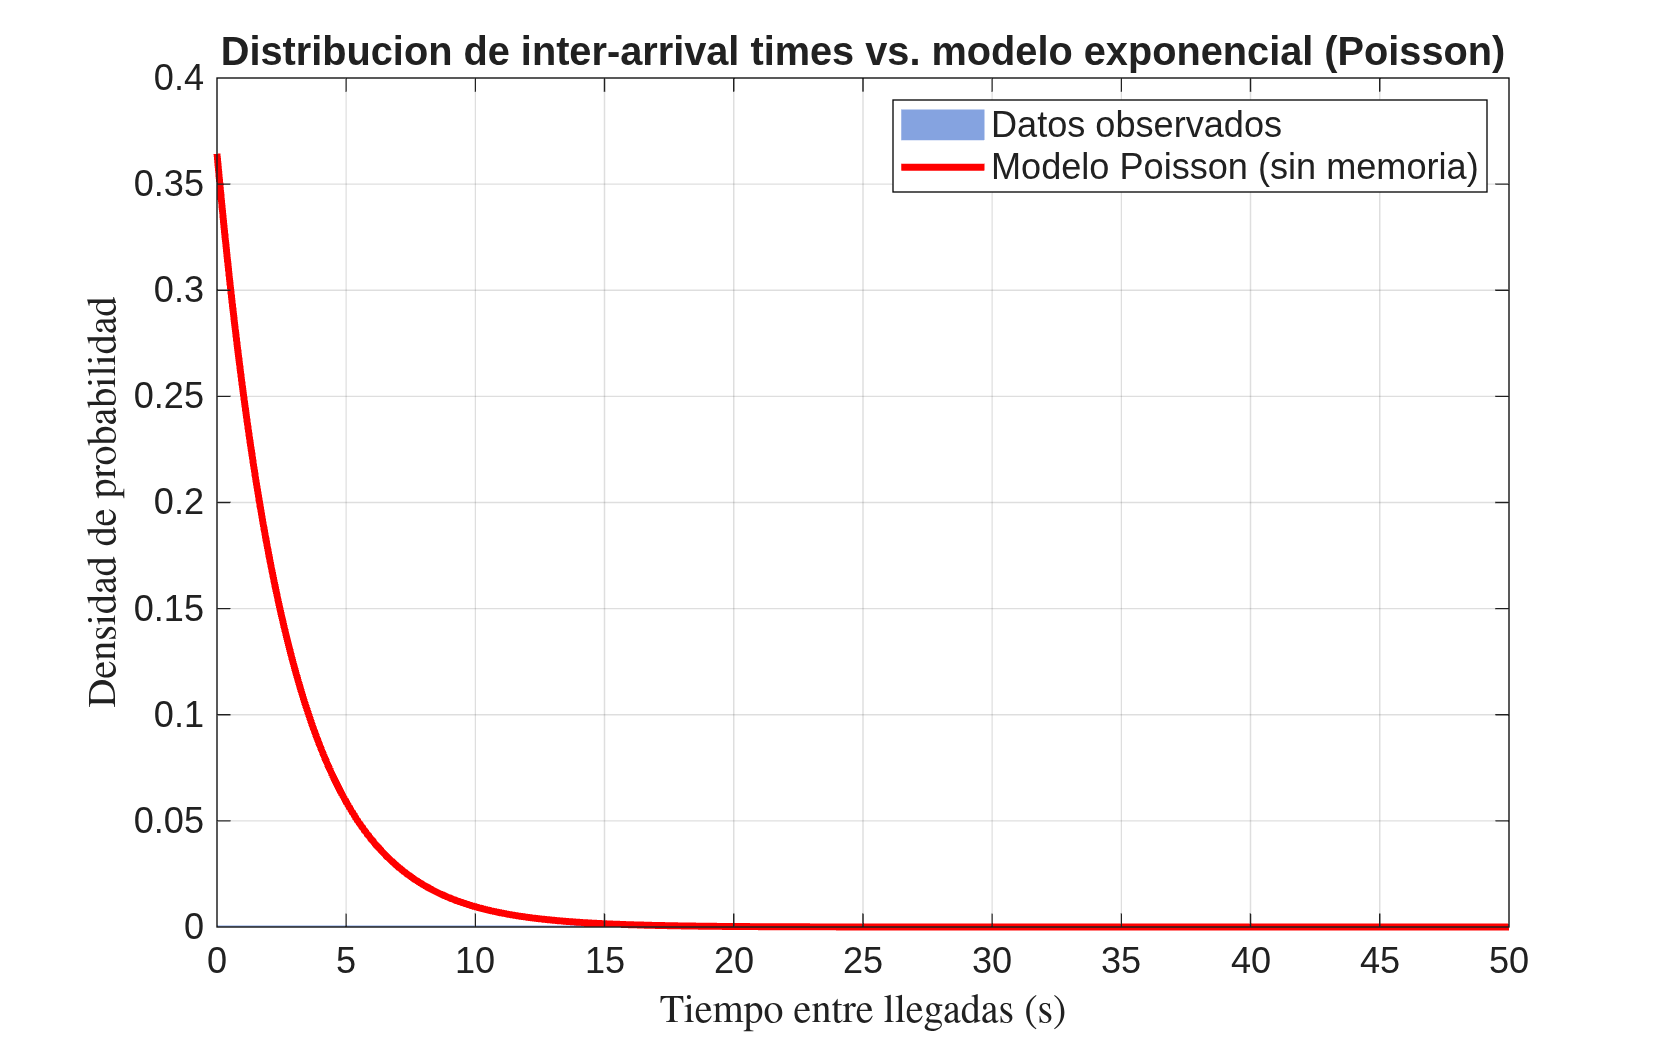
\includegraphics[width=\textwidth]{actividades/actividad6/imgs/histograma.png}
        \caption{Histograma de los inter-arrival times. La cola pesada
                 refleja la presencia de eventos de larga duración.}
        \label{fig:a6-hist}
    \end{minipage}
\end{figure}

Los estimadores VT y LD, así como el clasificador de la Actividad~4, se aplican
sin modificación metodológica, garantizando comparabilidad con los dominios
previos. Esta continuidad metodológica es esencial: permite situar el tráfico
NASA en el mismo espacio de parámetros que las secuencias sintéticas y las
señales cardíacas.

% ------------------------------------------------------------
\subsection{Estimación del parámetro de Hurst}
% ------------------------------------------------------------

El método Varianza--Tiempo arroja $\hat{H}_{\text{VT}} = 0{,}5435$ con
$R^2_{\text{VT}} = 0{,}9911$ e intervalo de confianza del $95\%$
$[0{,}5408;\,0{,}5462]$. El ajuste lineal del diagrama log-log es excelente,
confirmando que el escalamiento de varianza sigue una ley de potencias
consistente con dependencia de rango largo ($H > 0{,}5$).

El método Log--Escala obtiene $\hat{H}_{\text{LD}} = 0{,}5064$ con parámetro de
escala $\alpha = 0{,}0127$. La estimación es más conservadora que VT, en línea
con los hallazgos de las Actividades~1 y~3, donde LD exhibió mayor varianza en
muestras de gran tamaño con alta LRD.

\begin{figure}[H]
    \centering
    \begin{minipage}[t]{0.48\textwidth}
        \centering
        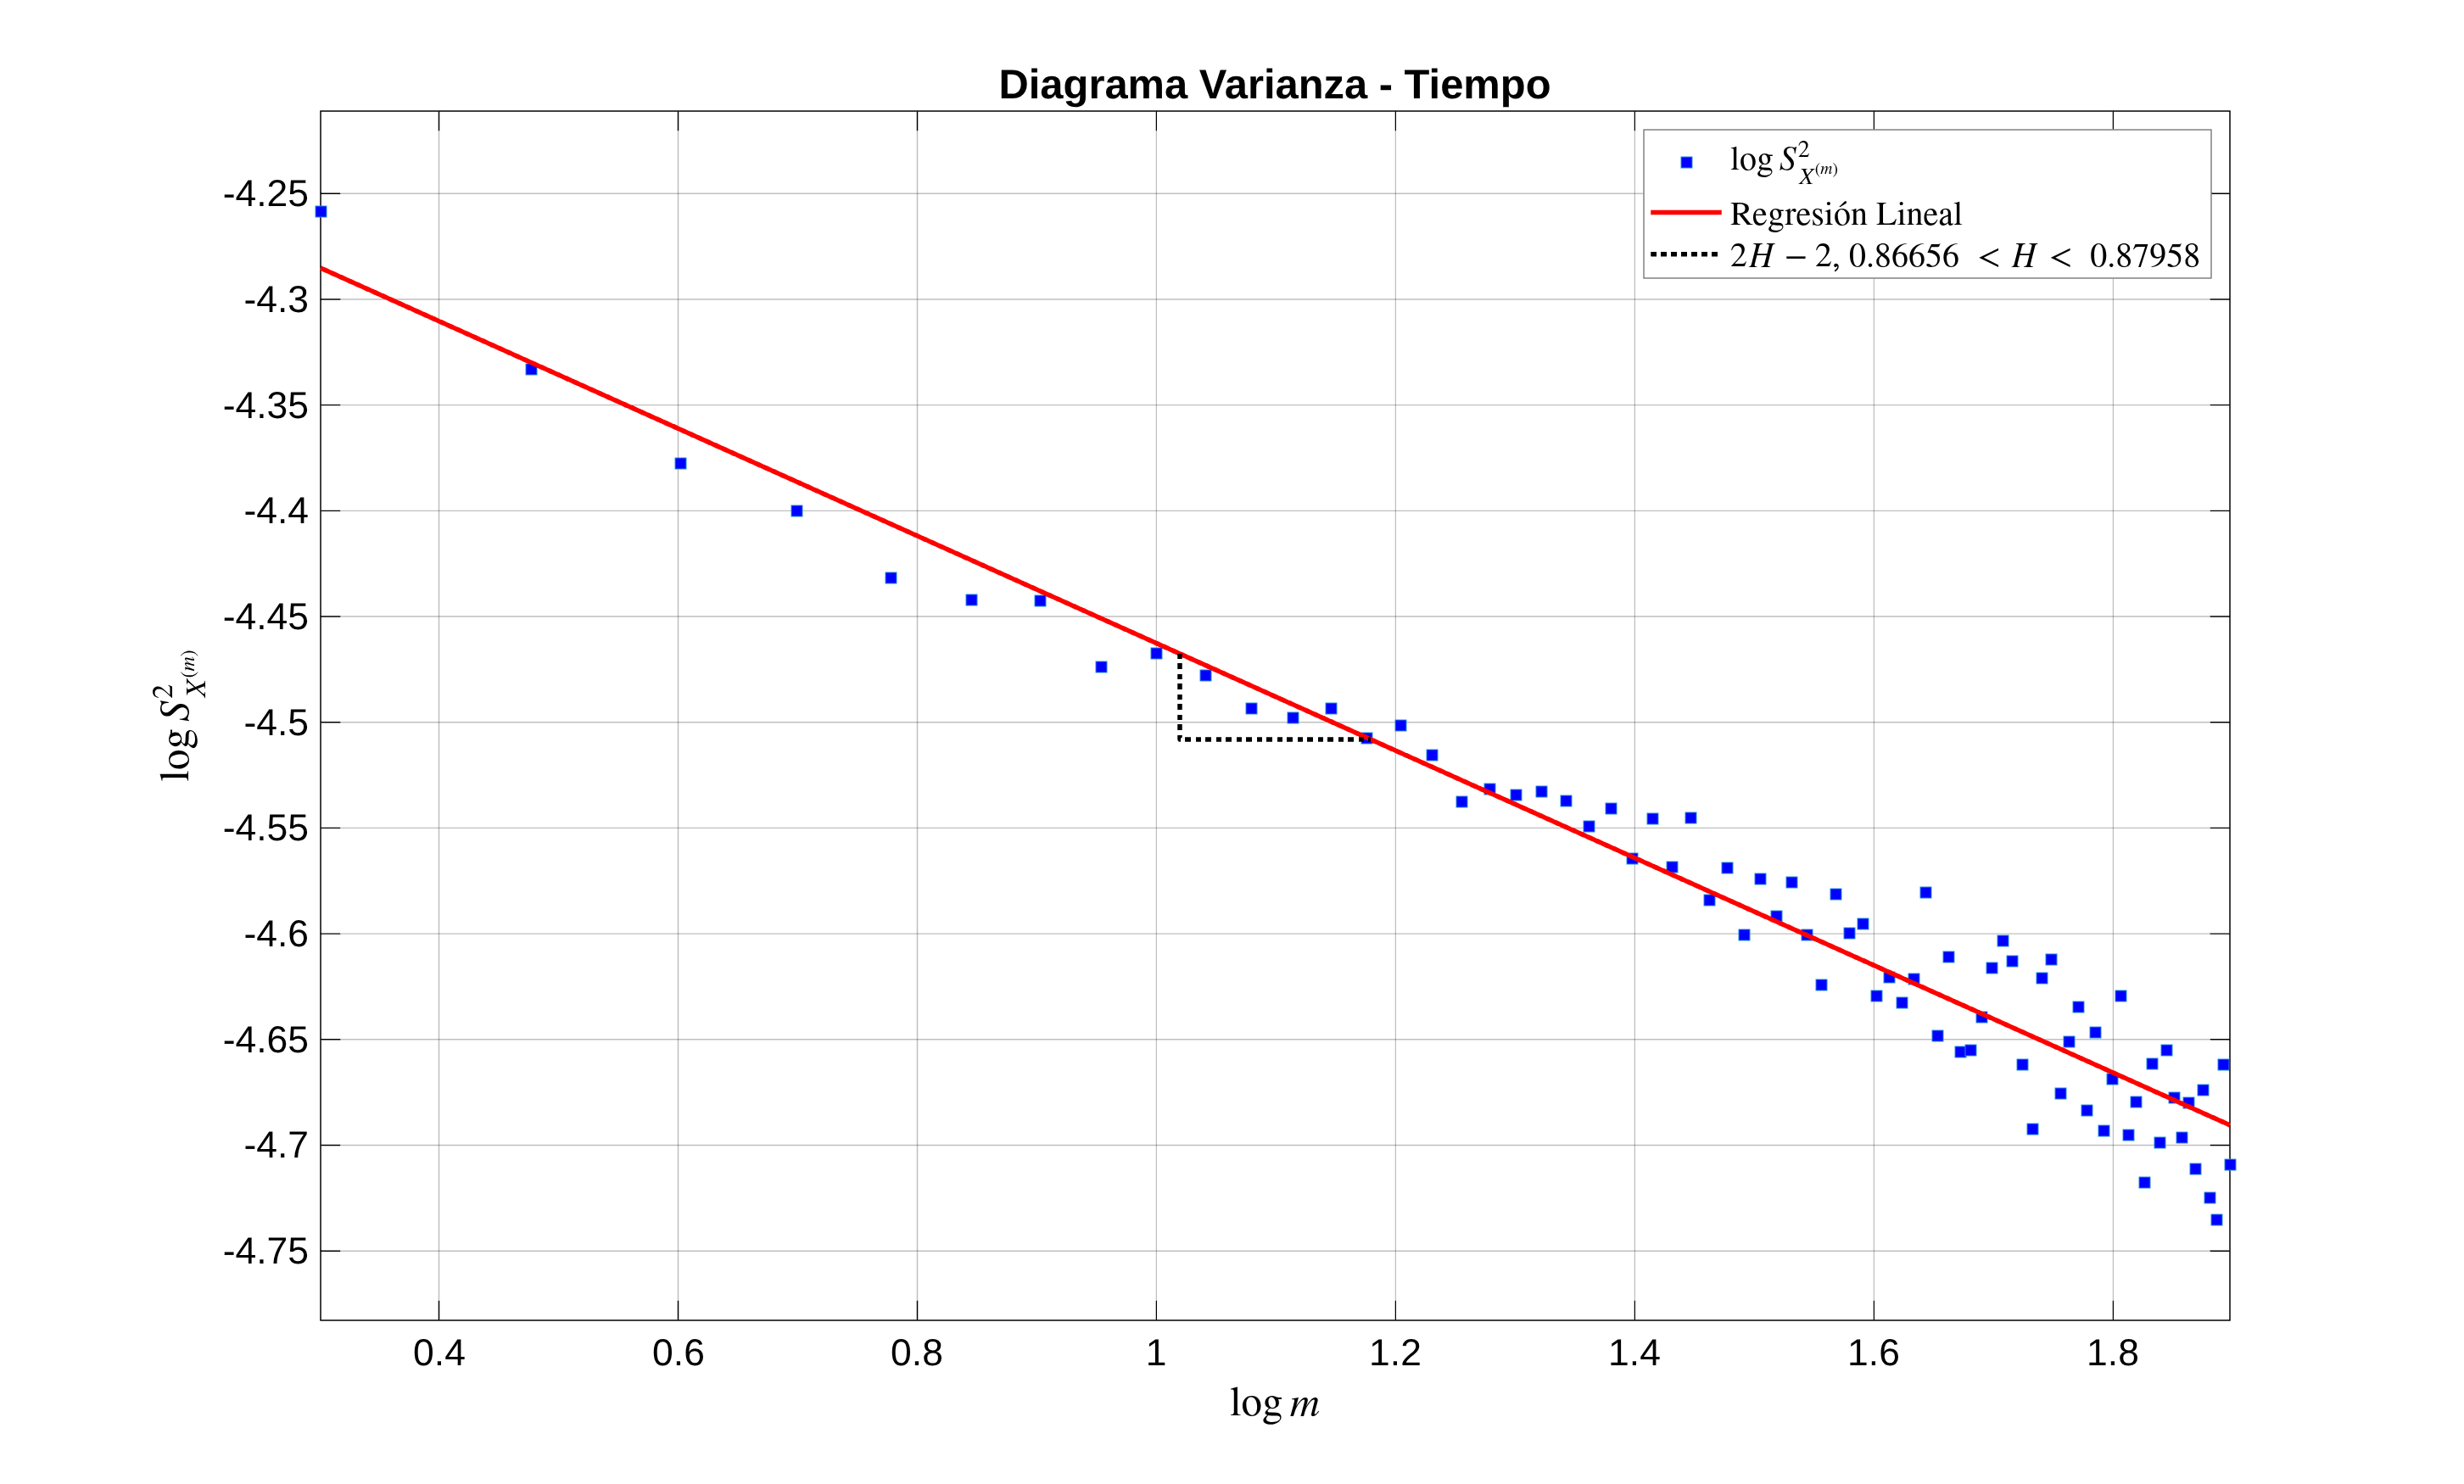
\includegraphics[width=\textwidth]{actividades/actividad6/imgs/diagrama_vt.png}
        \caption{Diagrama Varianza--Tiempo. La pendiente del ajuste lineal
                 determina $\hat{H} = 0{,}5435$, confirmando LRD.}
        \label{fig:a6-vt}
    \end{minipage}
    \hfill
    \begin{minipage}[t]{0.48\textwidth}
        \centering
        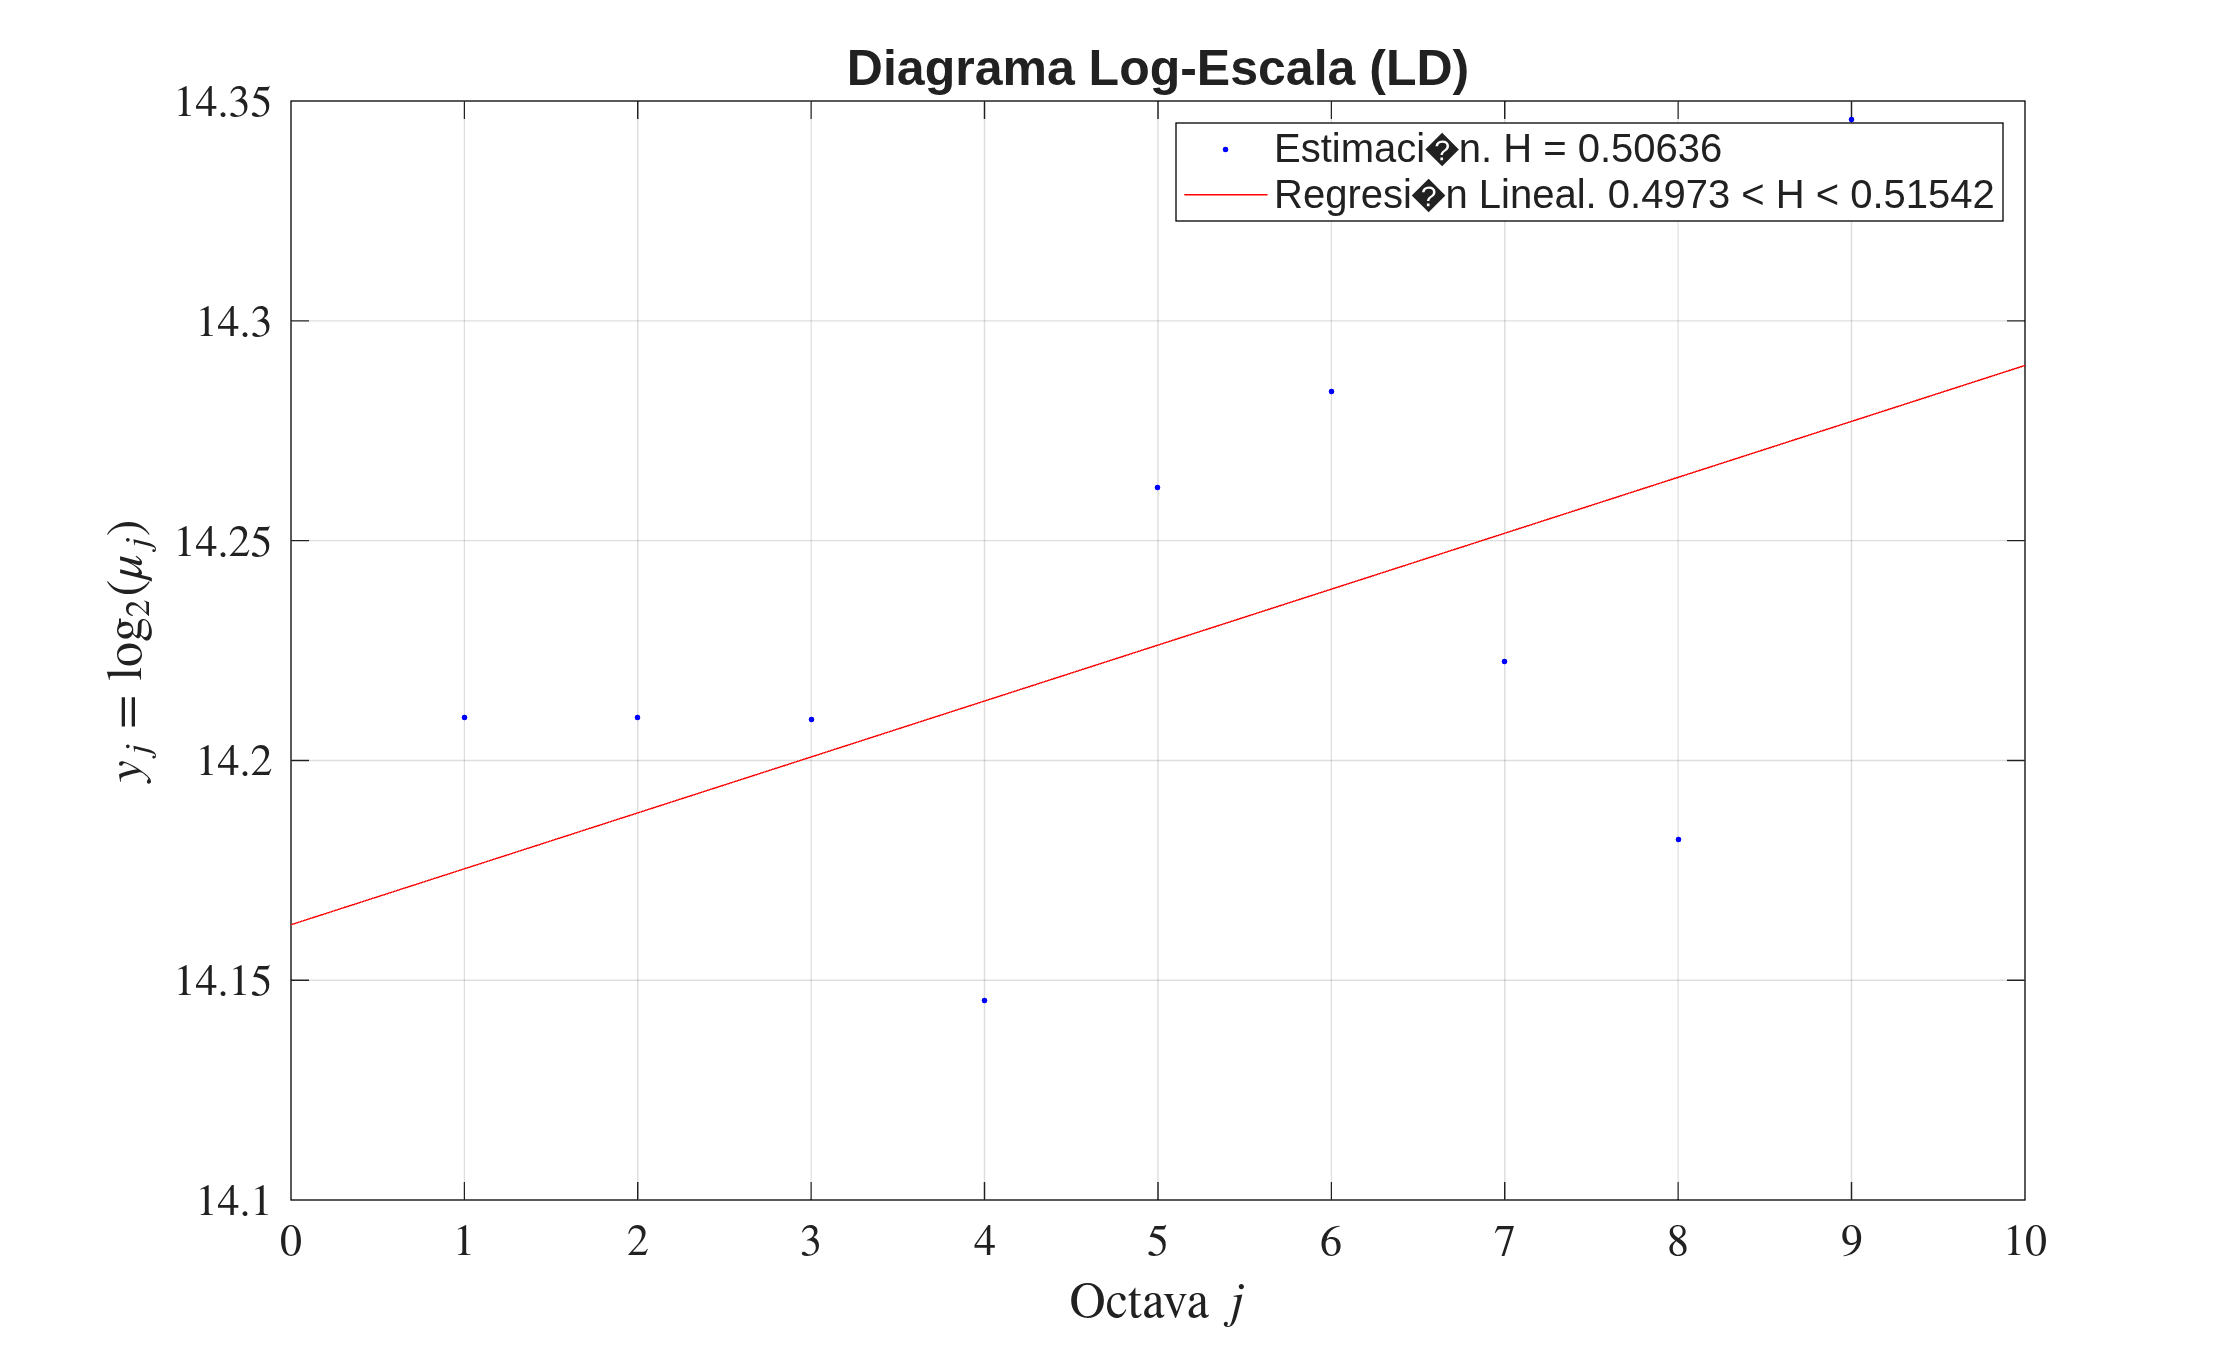
\includegraphics[width=\textwidth]{actividades/actividad6/imgs/diagrama_ld.png}
        \caption{Diagrama Log--Escala con wavelets de Haar.
                 Confirma LRD con $\hat{H} = 0{,}5064$.}
        \label{fig:a6-ld}
    \end{minipage}
\end{figure}

Ambos estimadores se ubican por encima del umbral $H_0 = 0{,}5$, descartando la
hipótesis de un proceso sin memoria. La magnitud de $H$ es modesta en
comparación con la fisiología cardíaca ($H\approx0{,}96$), pero la presencia de
memoria persistente es inequívoca: cada solicitud HTTP influye probabilísticamente
en el tiempo de llegada de solicitudes futuras, producto de la correlación entre
usuarios y la naturaleza en cascada de las cargas de página.

% ------------------------------------------------------------
\subsection{Clasificación mono/multifractal}
% ------------------------------------------------------------

Se aplicó el clasificador de la Actividad~4 al dataset NASA. La función de
escalamiento $\tau(q)$, obtenida mediante \texttt{dwtleader}, presenta curvatura
significativa con $R^2_{\tau} = 0{,}4808$, valor considerablemente inferior al
umbral de $0{,}95$ establecido para linealidad.

\begin{figure}[H]
    \centering
    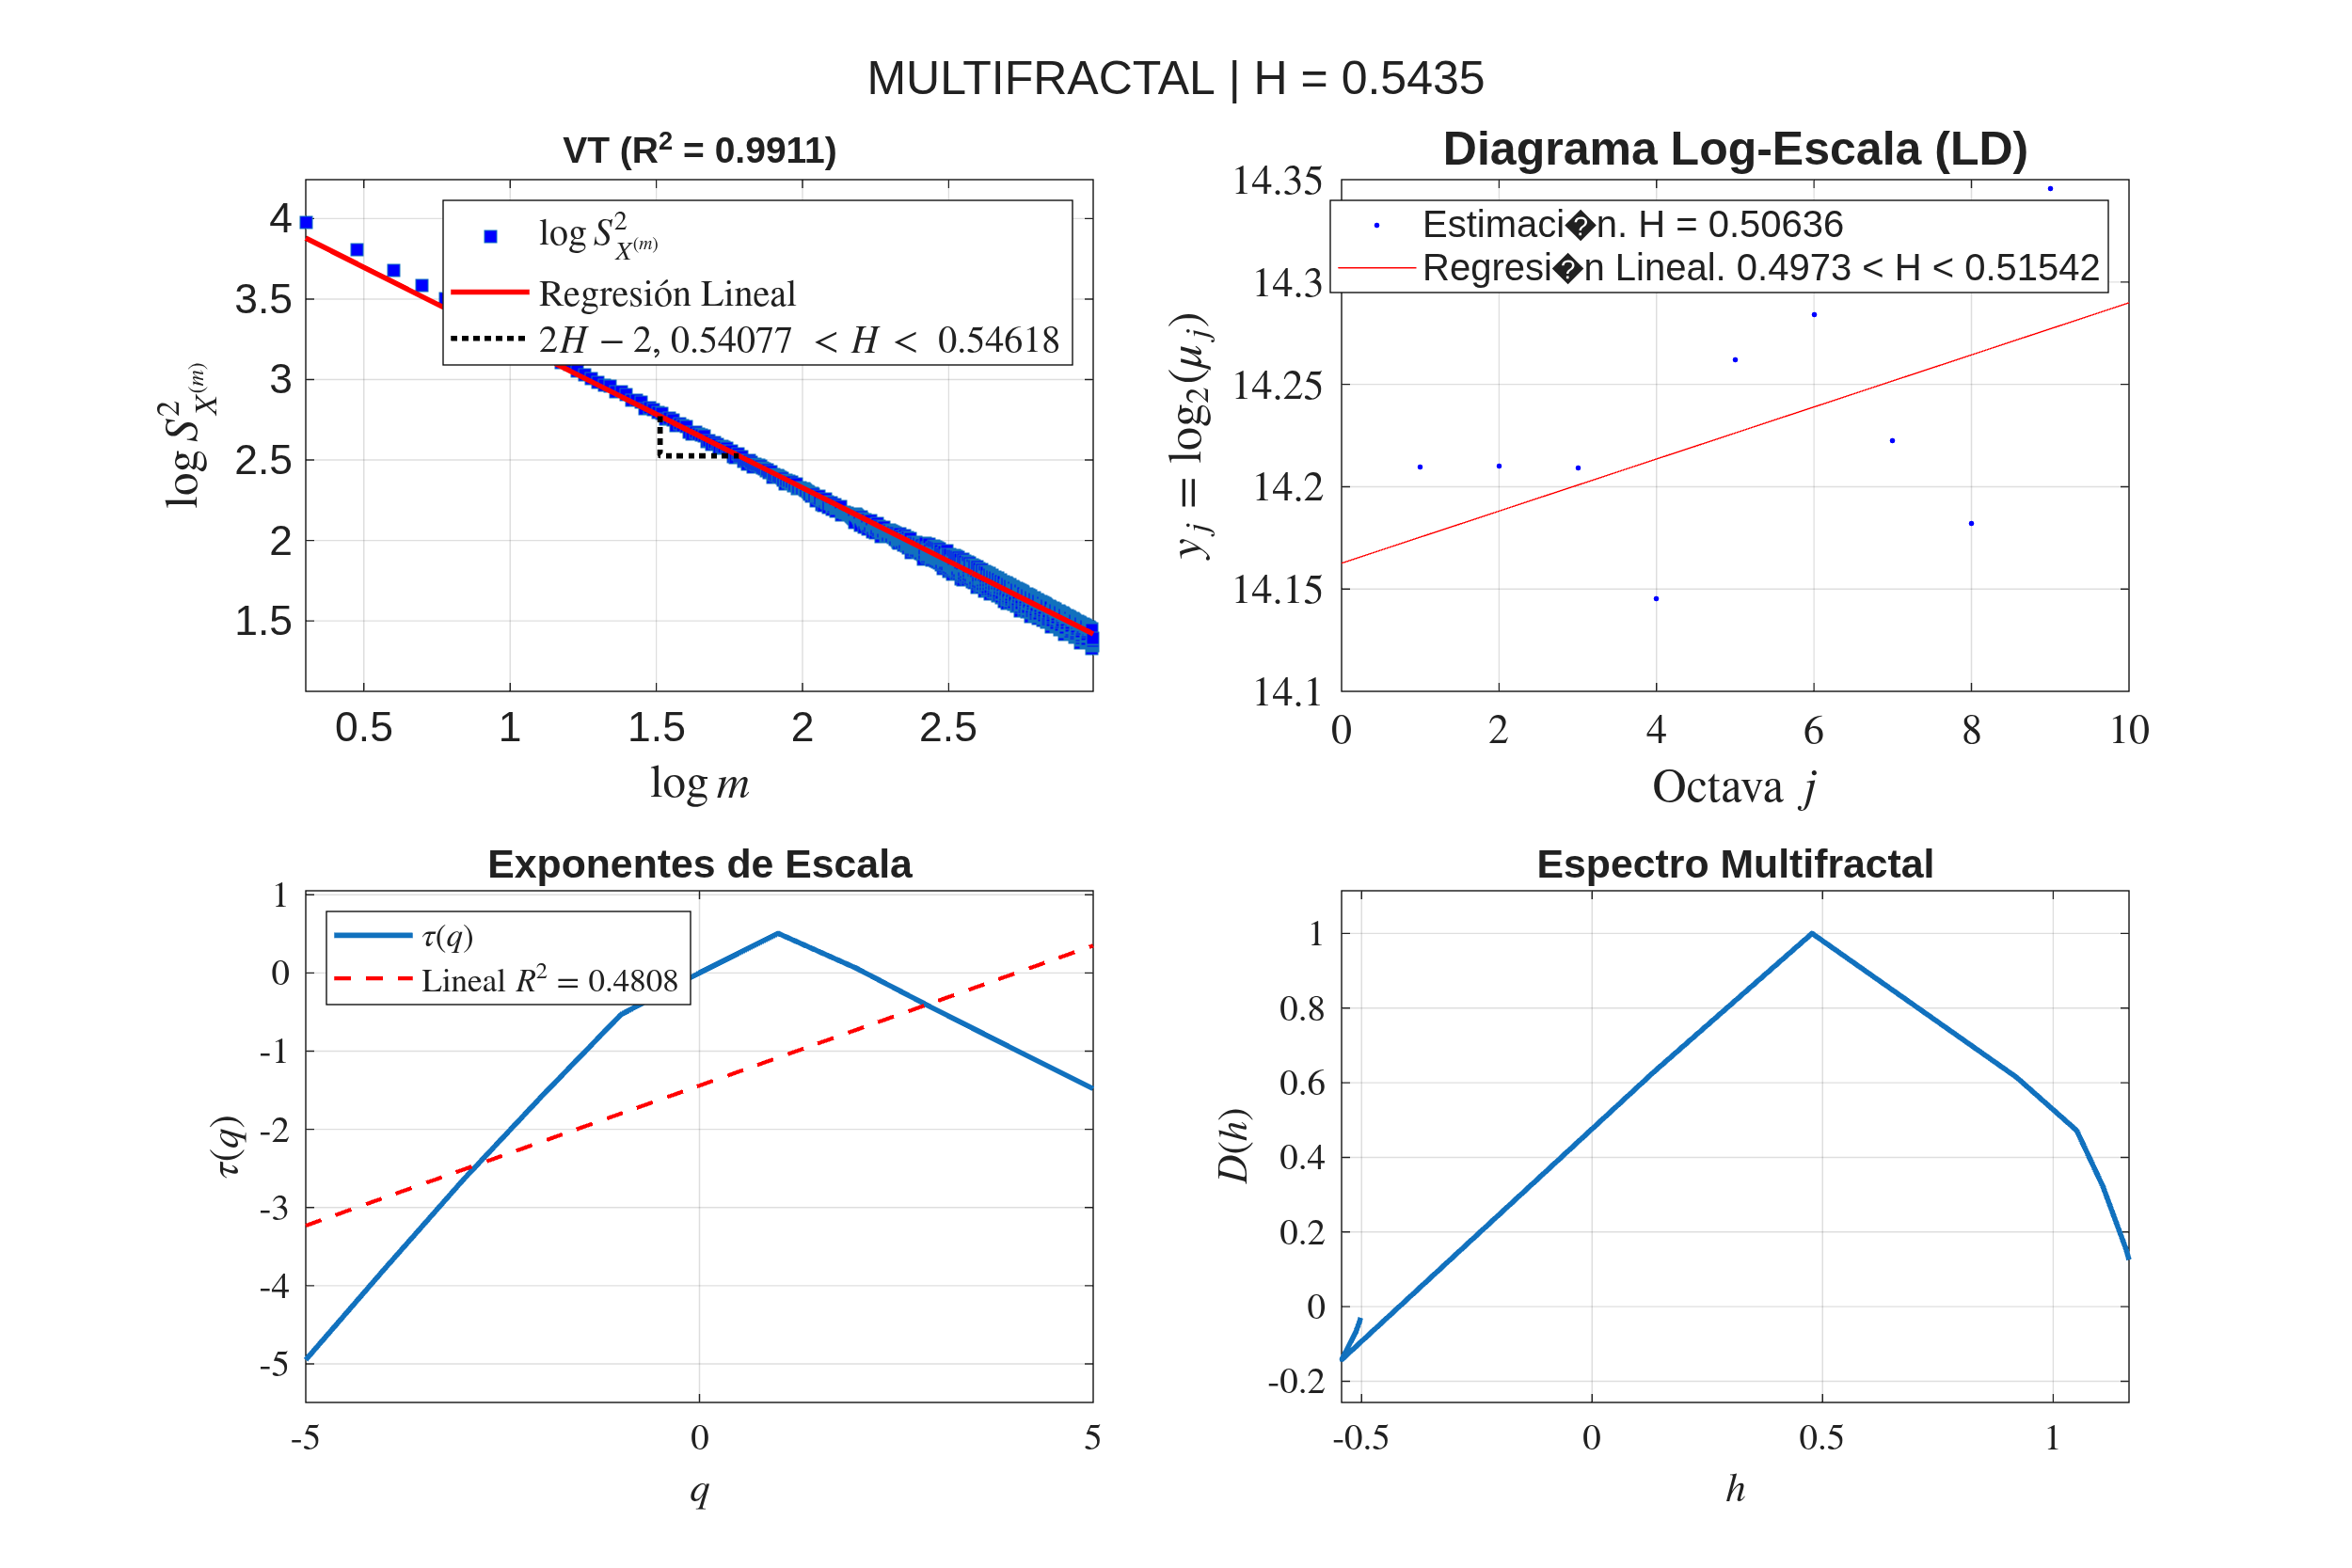
\includegraphics[width=0.88\textwidth]{actividades/actividad6/imgs/clasificacion_fractal.png}
    \caption{Clasificación del tráfico NASA. La curvatura de $\tau(q)$
             ($R^2_{\tau} = 0{,}4808$) confirma naturaleza multifractal.}
    \label{fig:a6-clasif}
\end{figure}

El tráfico NASA se clasifica como \textbf{multifractal}. Esto implica que no
existe un único exponente de escalamiento global; diferentes periodos de carga
(pico vs.~valle) poseen dinámicas de escalamiento local distintas. La
multifractalidad en tráfico web invalida modelos de colas con un único parámetro
para todo el rango operativo, dado que subestiman sistemáticamente la
probabilidad de ráfagas concurrentes y la magnitud de los picos de congestión.

% ------------------------------------------------------------
\subsection{Una taxonomía de dominios fractales}
% ------------------------------------------------------------

Los sistemas analizados en este trabajo pueden organizarse en un espacio
conceptual bidimensional donde el eje horizontal representa el grado de
dependencia de rango largo (de $H=0{,}5$ a $H\approx1{,}0$) y el eje vertical
la heterogeneidad espacial (de monofractal a multifractal). Esta taxonomía
revela una estructura común que trasciende los dominios de aplicación.

\begin{figure}[H]
\centering
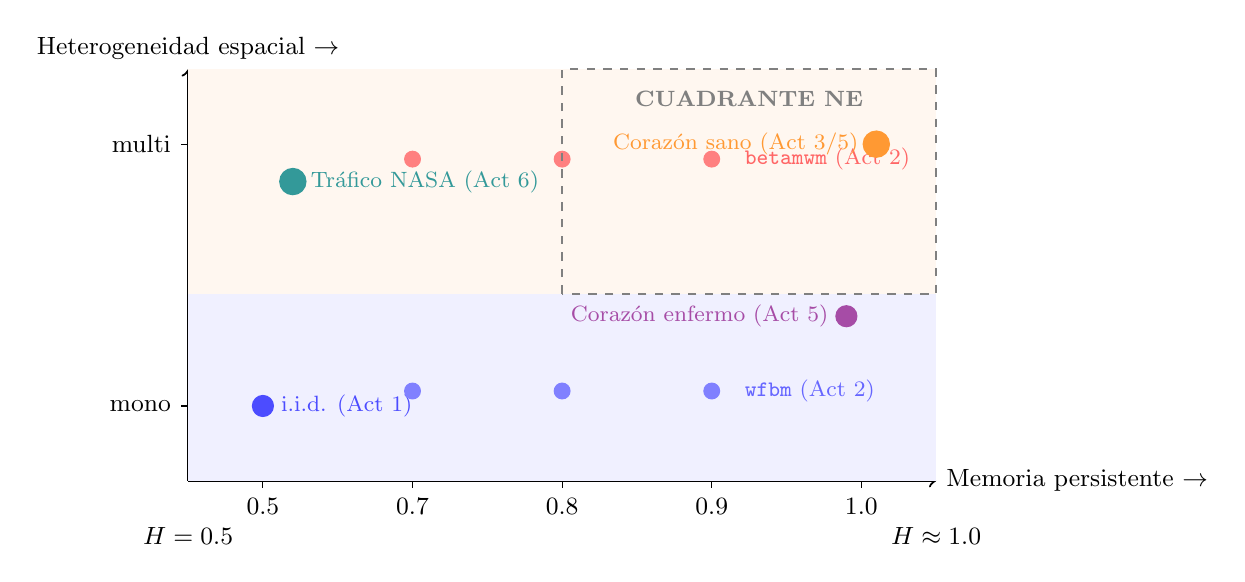
\begin{tikzpicture}[scale=0.95, every node/.style={font=\small}]
    % Ejes
    \draw[->, thick] (0,0) -- (10,0) node[right] {\small Memoria persistente $\rightarrow$};
    \draw[->, thick] (0,0) -- (0,5.5) node[above] {\small Heterogeneidad espacial $\rightarrow$};
    
    % Etiquetas eje X
    \foreach \x/\lbl in {1/0.5, 3/0.7, 5/0.8, 7/0.9, 9/1.0} {
        \draw (\x,0.1) -- (\x,-0.1) node[below] {\lbl};
    }
    \node[below] at (0,-0.5) {$H=0.5$};
    \node[below] at (10,-0.5) {$H\approx1.0$};
    
    % Etiquetas eje Y
    \draw (0.1,1) -- (-0.1,1) node[left] {mono};
    \draw (0.1,4.5) -- (-0.1,4.5) node[left] {multi};
    
    % Regiones
    \fill[blue!6] (0,0) rectangle (10,2.5);
    \fill[orange!6] (0,2.5) rectangle (10,5.5);
    
    % Puntos sintéticos
    \filldraw[blue!70] (1,1) circle (4pt) node[right=3pt, font=\footnotesize] {i.i.d. (Act~1)};
    \filldraw[blue!50] (3,1.2) circle (3pt);
    \filldraw[blue!50] (5,1.2) circle (3pt);
    \filldraw[blue!50] (7,1.2) circle (3pt);
    \node[right=3pt, blue!60, font=\footnotesize] at (7.2,1.2) {\texttt{wfbm} (Act~2)};
    
    % Puntos multifractales sintéticos
    \filldraw[red!50] (3,4.3) circle (3pt);
    \filldraw[red!50] (5,4.3) circle (3pt);
    \filldraw[red!50] (7,4.3) circle (3pt);
    \node[right=3pt, red!60, font=\footnotesize] at (7.2,4.3) {\texttt{betamwm} (Act~2)};
    
    % Tráfico NASA
    \filldraw[teal!80] (1.4,4.0) circle (5pt) node[right=3pt, font=\footnotesize] {Tráfico NASA (Act~6)};
    
    % Corazón sano
    \filldraw[orange!80] (9.2,4.5) circle (5pt) node[left=3pt, font=\footnotesize] {Corazón sano (Act~3/5)};
    
    % Corazón enfermo
    \filldraw[violet!70] (8.8,2.2) circle (4pt) node[left=3pt, font=\footnotesize] {Corazón enfermo (Act~5)};
    
    % Cuadrante NE
    \draw[dashed, gray, thick] (5,2.5) rectangle (10,5.5);
    \node[font=\footnotesize\bfseries, gray] at (7.5,5.1) {CUADRANTE NE};
\end{tikzpicture}
\caption{Taxonomía de dominios fractales. Los sistemas con memoria persistente
         y heterogeneidad espacial (cuadrante NE) incluyen tanto fisiología
         cardíaca como tráfico transaccional Cloud, revelando propiedades
         estructurales comunes. Los sintéticos puros ocupan la diagonal:
         \texttt{wfbm} es monofractal por construcción y \texttt{betamwm} es
         multifractal por construcción.}
\label{fig:taxonomia}
\end{figure}

Los dominios con memoria persistente y heterogeneidad espacial ---corazón sano
tratado en las Actividades~3 y~5, y tráfico web objeto de esta actividad---
ocupan el cuadrante noreste del mapa. A diferencia de las secuencias i.i.d.\ del
Actividad~1, que carecen de ambas propiedades y permanecen en el origen, estos
sistemas comparten tres características estructurales fundamentales:

\begin{enumerate}[leftmargin=2em]
    \item \textbf{Retroalimentación temporal.} El estado presente depende del
          pasado de forma no trivial. En el corazón, la regulación autónoma
          integra señales históricas del barorreflejo; en el servidor web, una
          solicitud activa cachés y conexiones persistentes que modifican la
          distribución de tiempos de llegada futuros.
    \item \textbf{Interacción multiescala.} Los procesos operan simultáneamente
          en escalas temporales distintas. La variabilidad cardíaca integra
          oscilaciones de segundos (respiratoria), minutos (barorreflejo) y
          horas (ciclo circadiano); el tráfico web superpone sesiones de
          usuarios individuales, ráfagas de contenido viral y patrones
          diurnos/nocturnos de uso global.
    \item \textbf{Heterogeneidad estructural.} Diferentes regiones o periodos
          exhiben dinámicas locales distintas. Los intervalos RR de un paciente
          con hipertensión (Actividad~5) muestran espectros de singularidad más
          estrechos que los sanos; los picos de carga del servidor NASA poseen
          exponentes de escalamiento diferentes a los valles de actividad.
\end{enumerate}

Esta convergencia estructural sugiere que la fractalidad no es un epifenómeno
del dominio biológico, sino una propiedad emergente de sistemas complejos con
retroalimentación, multiescala y heterogeneidad.

% ------------------------------------------------------------
\subsection{Análisis de la Actividad 6}
% ------------------------------------------------------------

El análisis del dataset NASA HTTP confirma que la fractalidad trasciende la
frontera entre sistemas biológicos y tecnológicos. El parámetro de Hurst
$\hat{H}_{\text{VT}} = 0{,}5435$ ($R^2 = 0{,}9911$) y
$\hat{H}_{\text{LD}} = 0{,}5064$ confirman dependencia de rango largo con
alta confiabilidad en el ajuste, mientras que $R^2_{\tau} = 0{,}4808$
establece la naturaleza multifractal del tráfico.

A diferencia de la fisiología cardíaca, donde la LRD es intensa
($H\approx0{,}96$) y está vinculada a la complejidad adaptativa del sistema
nervioso autónomo, el tráfico web exhibe una memoria persistente más modesta
pero igualmente significativa. La multifractalidad en este dominio tiene
implicaciones prácticas directas: invalida la hipótesis de llegadas de Poisson
que subyace a los modelos clásicos de teoría de colas, y exige estrategias de
provisionamiento dinámico que reconozcan la coexistencia de regímenes de carga
con distintas dinámicas de escalamiento.

La complementariedad entre VT y LD, observada sistemáticamente desde la
Actividad~1, se reproduce una vez más: VT ofrece una estimación más alta de $H$
con mejor ajuste lineal, mientras que LD proporciona una cota conservadora. Este
patrón es robusto ante cambios de dominio, lo que refuerza la recomendación de
utilizar ambos estimadores de forma conjunta en cualquier análisis de series
temporales con estructura fractal.

